% !TeX root = ../../thesis.tex
\chapter{Introduction}\label{ch:introduction}

\epigraph{"Blessed are the cracked, for they shall let in the light."}{--- Groucho Marx}

% \epigraph{"If free will does not exist, it would be necessary to invent it"}

Alan Turing's seminal 1950 paper ``Computing Machinery and Intelligence'' opens with a simple question: can machines think?
74 years later, a rigorous and formal definition of thinking, and intelligence in general, is still eluding us.
Reasoning, creativity, pattern recognition, problem solving, generalization, planning, optimization; while intelligence accepts a multitude of broad and imprecise definitions, when asked what are the definitive aspects of intelligence, ironically we cannot but self-referentially point to ourselves.
Furthermore, the advent of generative AI with its capability to model linguistic, reasoning, and creative capacities all the more closely, blurs the line even further between ``real'' and ``artificial'' intelligence, between the original and the simulacrum; could it be mere computation that goes on in our brains?
Besides the philosophical line of inquiry, there is immense -- and lucrative -- promise of \gls{AI} towards automating both menial and creative human activities \cite{benjamin1935work}, yet the hurried and uncritical adoption of \gls{AI} solutions contains considerable risks.

Today, a wide range of systems employ \gls{AI} to detect, classify, or infer on data, a range that will only keep expanding.
Approached generally, these systems perform some form of decision-making in the enviroments they reside: based on their observed inputs, they produce a range of outputs that are directly or indirectly communicated back to the user.
Without being exhaustive, such AI-enabled systems include malware, bot, fraud, and intrusion detection, facial recognition, credit scoring, autonomous vehicles, image classification, and more recently any system powered by LLMs: from code generation to customer service.
No matter how statistically prevalent, all of these environments contain adversaries.
Therefore, for systems that expose public interfaces a false sense of security can be disastrous, as multiple threats can induce erroneous decisions and prevent the \gls{AI} models from behaving according to their specification.
One such threat is the thriving and of increasing sophistication bot activity online.
Such automation is often powered by AI, while the sole methodology for demarcating humans and machines still originates from that 74 year old paper, the Turing Test.
Also known as the imitation game, Turing tests have been widely deployed online as Captchas to hinder bots and automation.
Yet the Turing test is no longer an adequate approach, as the burgeoning \gls{AI} capabilities are rapidly phasing it out of relevance.

% Captcha is just one type of AI-based system that faces adversarial threats.
In this dissertation we explore the security and correct functioning of AI-based systems under attack, one of them being Google reCAPTCHA.
Concretely, we scope on decision-based evasion attacks, a pervasive type of threat that these systems face when exposed to the real-world, and explore potential defenses and mitigations.
In an ever-changing landscape of threats and mitigations, adversaries as well as defenses have to constantly adapt to stay at the top of their game.
The systems we investigate are situated in three distinct domains that also represent diverse modalities: bot detection, malware detection, and image classification.
While image classification might initially appear a less relevant domain for cybersecurity, and in some regards it is, it still is the domain where all foundational \gls{AML} research is performed.
In the sections that follow, we introduce the aforementioned attacks and defenses in each domain we investigate, as well as what actually means to be ``adaptive''.

\section{Adaptive Attacks and Defenses}

Networked systems have historically been vulnerable to multiple types of attacks, from DDoS and malware to spoofing and packet sniffing.
It comes as no suprise then that the environments modern AI-based systems inhabit are inherently adversarial.
One key difference however is that, besides the threats existing at various communication (\gls{OSI}) layers, they now have to additionally reckon with threats at the logical level, specifically through the information that their \gls{AI} models process as inputs.
Even when the models' decisions are not directly divulged to the user, like in the case of reCAPTCHA v3, they inadvertently constitute feedback.
If additionally these systems can be consistently queried, a feedback loop is created that adversaries can use to \textit{adaptively} control their attacks~\cite{astrom1995adaptive}.
Defenses on the other hand have been consistently ineffective or bypassed, something that gave rise to a methodological shift in the robustness literature: no defensive results are reliable unless the evaluation is performed with \textit{adaptive} attackers~\cite{madry2017towards}.
Note the dual use of adaptive here; in \gls{AML}, “adaptive” by convention refers to attacks with full knowledge of how a defense works and the tools to bypass it.
In this dissertation, we expand the term to include adaptive control, defined as the ability of a system to self-adapt: automatically reconfigure and optimize itself in response to feedback received from the environment.
In all the three domains we investigate, we discover that adaptive adversaries, in the comprehensive sense we introduce, pose a much higher threat than their non-adaptive versions do.

Defensive \gls{AML} research is often confounded by a clear conflict of interest, namely how much effort is made in adapting and optimizing any attacks employed.
Furthermore, it often happens that attacks and their parameters are suboptimal out-of-the-box when applied in different environments~\cite{croce2020reliable}.
Finally, adversaries might apply evasive actions on the the input -- for instance transformations the model is invariant to -- with the goal to bypass active defenses~\cite{chen2020stateful,li2022blacklight}.
As the performance of an attack and how evasive it is to detection are two properties in trade-off, they are non-trivial to combine.
For the three aforementioned reasons we discover that, unless attacks are performed in a \textit{fully} adaptive manner, any results on the empirical robustness are unreliable and incomplete.
For a thorough and representative evaluation then, the first step is to turn adaptive any attacks employed.

The second step is to ask if the same can be done for defenses.
The state-of-practice and most widely used defense, irrespective of domain or modality, is adversarial training.
Adversarial training constitutes a counterfactual investigation on the inputs of the model, and before or during the training of a model it asks the following question: what are all the \textit{valid} ways that something could be different, and still be the \textit{same} thing.
Perceived differently, adversarial training is a deliberate \gls{OOD} investigation, under the specific structural and variational constraints that have to be respected and are not shared between domains.
Adversarial training is typically performed in white-box fashion, meaning that the input perturbations are computed through the gradients of the model's computational graph in an end-to-end fashion.
Even if we assumed full white-box access to the model and its analytical expressions, any discontinuity makes the computation of gradients impossible, from a simple argmax in next token prediction to the prominent gap between problem and feature (representation) spaces that some domains have.
In our work we discover that in such domains it is preferable to perform adversarial training through the problem space while respecting the constraints that the domain has, as it outperforms gradient-based solutions.
Not only that, but given well-defined adversarial capabilities we can additionally guarantee a probabilistic level of robustness against them.
This is a significant step beyond how adversarial training is performed, as until now the robustness that it confers was merely empirical.

Finally, in the case of image classification, we discover that adversarial training offers some limited and unsatisfactory robustness.
As models cannot update their decision boundary in an online manner and in response to
any adversarial activity on their interface, there exists a \textit{complement} to model hardening: active defenses, such as rejection and misdirection.
The intuition here is that the manner in which the model \textit{responds} has a complementary potential to what it has \textit{learned}.
This gap between the practical and theoretically possible robustness to decision-based attacks is the locus where our distinct from model hardening, active and adaptive defense emerges.
In a wide range of image classification models and attack plus defense scenarios, we demonstrate that active defenses are necessary complement to model hardening when facing decision-based attacks; then how these defenses can be circumvented by adaptive attacks, to finally elicit active and adaptive defenses.

\section{The Imitation Game}

Traditionally, Captchas have employed explicit challenges that only humans could solve.
At some point however, these challenges became more difficult to solve for humans than for automated methods based on \gls{AI}.
Thus recently a paradigm shift took place where newer Captchas ditched the ``puzzle'' approach and instead focused on behavior in order to tell humans and machines apart; the challenge was still there, but now implicit rather than explicit.
Ironically, such challenges or puzzles assist in the progressive refinement of the very thing they were designed to defend against: as the detection get better, so does the imitation.
In the long and recurring cycle of Captchas being introduced and broken, reCAPTCHA v3 by Google is the first to change the rules of the game: while before the nature of the challenge was explicit in the form of a puzzle or test, now it was obfuscated through the observation of undisclosed behavioral variables.
Security through obscurity however does not last; Google reCAPTCHA v3, a widely adopted real-world defense against bots, can be easily bypassed.
Moreover, as we will further demonstrate later, the detection tool itself can function as an instructor for perfecting the imitation of human behavior, with weak assumptions on the adversary.

In our first work, we perform the first comprehensive study of reCAPTCHA v3 along with its advanced risk analysis system, and build an automation framework for browsing websites through the graphical user interface.
This framework is powered by three different types of RL-based agents, each more capable than the previous in simulating human behavior on the web.
We host our own testbed website protected by reCAPTCHA v3 in order to first evaluate the extent that it can be exploited, and then provide to our methodology the signal that it can learn on: the score that our automated activity receives on the website.
Subsequently, we scale up our experiments to two actual websites that are not under our control and with considerable daily traffic, in order to evaluate how well our approach transfers and generalizes out of the testbed.
Over a period of fifteen months in various web environments and a wide range of experiments, we show that it is possible to for our automated solution to consistently avoid detection by reCAPTCHA v3.
Furthermore, we show that an adversary can exploit the implicit challenge itself in order to learn a web browsing behaviour that flies under the radar of the most widely used automation detector at the time.
Finally, we perform a state-of-the-art explainability approach to quantitatively evaluate how different factors of our automation tools influence the score.

As Captchas are transitioning towards behavioral aspects, and as AI capabilities are becoming more comprehensive, the competition in differentiating between human interaction and its imitation accelerates.
Such imitation however, no matter how refined and identical to human, would be a stretch to claim that is the result of intelligence or cognition.
Rather, one would be correct in pointing out that it was indistinguishable for the discriminative model under question.
Therein lies the main limitation of telling humans and machines apart through discriminative methods: given sufficient modeling capacity and computation---both of which have been scaling extremely well so far---the competition between imitator and detector will eventually favor the former.
From the connectionist and computationalist views, cognition and consciousness can be viewed as emergent properties of neural activity, yet the tremendous contemporary progress on \gls{AI} has arguably brought us no closer to uncovering the mysteries of intelligence.

\textbf{Publication Data:} \fullcite{tsingenopoulos2022captcha}

\section{From Imitation to Evasion}

Researchers are ever eager to investigate challenging suppositions, even when these are loosely grounded to and unrepresentative of reality.
It did not come as a surprise then that initially all adversarial attacks on \gls{ML}, and therefore defenses too, were performed on image classification models.
The main reason behind the almost exclusive focus of adversarial attacks on image classification models  is the ease and immediacy of performing them, making them ideal choices for quick and prolific output.
This ease stems from the complete absence of a gap between the so called problem and feature spaces \cite{pierazzi2020intriguing}: whatever adversarial gradients are computed through the model, they can be applied directly on the input space, the images themselves.

Additionally, there are few constraints on what and where is changed, besides the total amount of perturbation.
These properties made image classification conducive to adversarial attacks, but in reality such a threat model is unrepresentative of every other domain.
This represented a disparity between the adversarial research being conducted, that is on feature representations, and more pragmatic lines of inquiry:
adversarial attacks against real-world, AI-based systems are \textit{necessarily} performed through the problem space.
As the objective of performing attacks is to render AI-systems robust and trustworthy, it follows that a clear assessment of vulnerability can only be achieved by performing and defending against attacks through the \textit{problem space}.

Secondly, the advent of adversarial examples precipitated a fundamental shift on how we perceive the generalization promise of \gls{DL}, forcing researchers to reckon with what are these models \textit{actually} learning.
The accelerating progress in \gls{AI} is supported by two primary pillars: data and computation.
As a result of collecting and curating them however, data inexorably contain artifacts and spurious correlations between dependent and independent variables, otherwise known as shortcut features \cite{geirhos2020shortcut}.
This phenomenon poses a considerable obstacle in deploying naively trained models in security critical domains that willfully collect data, as these shortcut features will be present and can be used for evasion.

Malware detection in particular has historically been vulnerable to both evasion and spurious correlations, vulnerabilities that are further aggravated by adopting ML-based solutions.
In our second work and in a broad collaboration between multiple universities and industrial partners, we investigate the \gls{AI}-based module of a widely known commercial antivirus, with the objective to harden it against adversarial malware.
Adversarial training as is conventionally applied was not applicable,
Adversarial training, the most reliable defensive technique is not applicable out of the box in this domain, for the principal reason that gradient-based perturbations rarely map back to feasible problem-space programs. 
We introduce a novel \gls{RL} approach for constructing adversarial examples, to subsequently adversarially train the model against evasion.
Our approach comes with two key advantages: a) it performs modifications that are feasible in the problem-space, and only those, thus it circumvents the inverse mapping problem, and b) it also makes possible to provide theoretical guarantees on the robustness of the model against a particular set of adversarial capabilities.

We collected an extensive dataset of benign and malicious binaries in order validate our theoretical insights.
Through our empirical evaluation, we arrive to two important and related results.
First, that \gls{ML} models and no matter their architectural innovations, are acutely vulnerable to adversarial attacks when naively trained on what data is available.
Secondly, that with our offensive approach and a few adversarial retraining iterations we can consistently diminish the success rate of the attack to 0\%.
Our results highlight the importance of performing adversarial training before any ML-based component or system goes into production.
In that way we demonstrate that constructing realistic and representative adversarial examples is not a mere academic exercise, but that also functions as concrete methodology for deploying intelligent systems robust to real-world adversaries.

\textbf{Publication Data:} \fullcite{tisngenopoulos2024train}

\section{From Adaptive Attacks to Adaptive Defenses}

As detection mechanisms improve, so do the imitations.
And as adversarial examples have illustrated, what makes something, \textit{something}, can be more elusive than we might be inclined to think; only through the constant interrogation of what is known, essence slowly reveals itself.
Neither of these conclusions is novel or surprising, yet such competition emerges intrinsically in diverse domains at the intersection \gls{AI} and computer security, from \gls{GAN}s and game theory to adversarial examples and adversarial training.

A recent hypothesis postulates that intelligence, and all its associated abilities, are the direct results of reward pursuing agency \cite{silver2021reward}; a reformulation of the Von Neumann–Morgenstern utility theorem~\cite{von1947theory}.
Naturally, this reward cannot be pursued from the environment unstrategically and irrespective to other agency in it.
This is something that in an exhaustible world has often brought intelligent agents at odds with each other, and even with their own continued survival~\cite{tohme2019superrational}.
Our directed intentionality towards the world combined with our expected utility maximizing agency, have been instrumental in developing our cognitive and critical faculties, but the capacity to be agents of our own undoing as well~\cite{rlblogpost, skalse2022defining}.

Let us now ground how this pursuit of reward connects to our work from a technical perspective.
So far we have introduced an adaptive attack against a real-world system, and an adaptive attack against a real-world system that subsequently is utilized to harden it against evasion.
In both cases, the adaptation and ultimate success of the attack is conditional on a reward signal emitted by the environment, information that even when attempted to be minimized is inadvertently emitted by all decision-making black-boxes.
Notably, that sparse and binary signal \textit{suffices} for attackers to adapt successfully.
As anticipated however, there the missing piece to the puzzle here, namely the counterpart to the adversarial agency in the form of adaptive defenses.
To that end, in our third work we first interrogate the property of being adaptive, then explore adaptive attacks \textit{and} then defenses in their interdependence.

In \gls{AML}, the canonical approach in robustness evaluation calls for adaptive attacks.
But how is the term ``adaptive'' precisely meant here?
That is with complete knowledge of the inner workings of a defense, as well as with all the available tools to bypass it~\cite{tramer2020adaptive}.
We introduce a more expansive notion of adaptive that includes adaptive control \cite{aastrom2013adaptive} and show how attacks but also defenses can benefit from it \emph{and} by learning from each other through interaction.
One could not overemphasize this: to reliably measure the robustness of a model, it is important to evaluate against both realistic and worst-case attacks.
We thus augment both attacks \emph{and} the evasive arsenal at their disposal through adaptive control, and do the same for the defenses, before we evaluate them first apart and then jointly under a multi-agent perspective.
We discover that active defenses, which control how a system responds, are a necessary complement to model hardening when facing decision-based attacks; then how these defenses can be circumvented by adaptive attacks, only to finally elicit active \emph{and} adaptive defenses.

We validate our observations through a wide theoretical and empirical investigation to confirm that adaptive adversaries pose a considerable threat to ML-based systems, even with merely black-box access, and that adaptive defenses are a necessary countermeasure.
% rekindling the proverbial arms race where defenses \emph{have} to be AI-enabled too.
In our work we demonstrate how our approach outperforms both attacks and defenses that are state-of-the-art, while bringing the offensive and defensive methodologies together to render effective insights over the robustness of real-world deployed ML-based systems.

\textbf{Publication Data:} \fullcite{tsingenopoulos2023adversarial}

\section{The Broader Picture}
% \section{Other Contributions}

This section serves as a means to put the three major research contributions in perspective, how they came to be research questions in the first place, how they connect with each other, and finally to present other related research results and activities.
As researchers, we are often motivated by a powerful but often unstructured drive to understand how things work.
It was in 2017, and before I even considered pursuing a PhD, that out of curiosity and happenstance I had the fortune to read the first paper that subsequently sparked the whole field of \gls{AML}: ``Intriguing Properties of Neural Networks''~\cite{szegedy2013intriguing}.
At the time, adversarial examples were a puzzling novelty, and I was instantly absorbed by their straightforward but elegant formulation and the perplexing phenonmenon.
This knowledge compelled me to pursue a more rigorous and deeper understanding of these admittedly intriguing properties: why, where, and how they happen.

When I intially started working on \gls{AML}, I discovered a prevalent shortcoming in almost the entirety of the related work: unrealistic assumptions on the level of access the adversary has to the model.
The vast majority of the attacks, and therefore defenses too, where assuming white-box access; an threat model that is completely unrepresentative for real-world deployed AI-based systems.
While white-box access is typically considered a given from the defensive perspective, this is not always the case for the offensive. Specifically, there are three prominent reasons why white-box, gradient-based attacks face serious challenges and limitations in realistic scenarios:

\begin{itemize}
    \item Many models have discontinuities in their closed-form expressions; a simple argmax -- for instance in modern autoregressive LLMs -- or merely having discrete outputs, suffices to render a model non-differentiable.
    \item Even when a model would be end-to-end differentiable, practical attacks when performed in the real-world are confounded by the non-invertibility of the feature perturbations back to the original object that these features represent.
    \item Finally, as model size and complexity increase, it quickly becomes intractable to interpret what these models actually learn solely based on the gradients, without using some form of higher-order features or concepts that are semantically meaningful in the problem space~\cite{kim2018interpretability}.
\end{itemize}

\begin{figure}
    \centering
    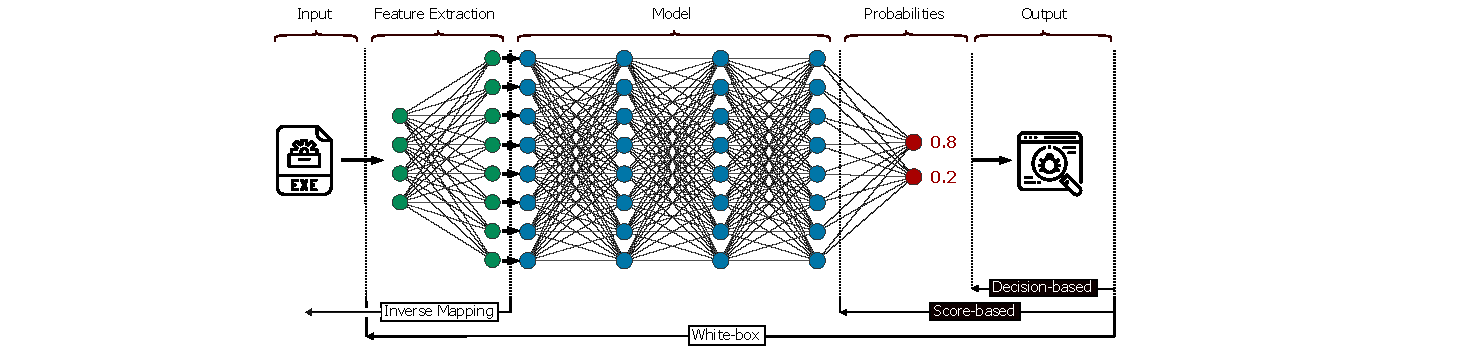
\includegraphics[width=0.99\textwidth]{pipeline.pdf}
    \caption{Abstract neural network based malware detection}
    \label{fig:pipe}
\end{figure}

Due to the aforementioend reasons, there are domains and use cases where performing the attacks through the problem space is preferable, and can lead to a more principled understanding of the vulnerabilities present.
To illustrate the distinction between problem-space and feature-space attacks, as well as situate them in a practical use case, \autoref{fig:pipe} depicts the full pipeline of a general malware detection model.
It starts from the sample as it occurs in the problem space, followed representation in the feature-space, the model, to the probabilities in $[0,1]$ and the decision space $\{0,1\}$.
The leftward arrows under the pipeline indicate the varying degrees of access an adversary can have.
Black-box attacks are further divided into score-based and decision-based depending on the access of the adversary to the model, the probabilities or just discrete decisions respectively.
White-box attacks on the other hand, have a full closed-form description of the model up to the feature representation.
Finally, the inverse mapping is a non-trivial challenge that confounds all domains where a gap between the problem and the feature space exists.

For real-world deployed models or systems, decision-based atatcks used to represent and still are the most realistic form of attack.
My work has thus opened lines of inquiry that primarily focused on black-box and decision-based attacks, with the ultimate objective to make models robust to them.
It quickly became apparent that when operating in black-box environments, which cybersecurity contexts typically are, then for a rigorous evaluation of a system's vulnerability we \textit{have to} optimize any attacks employed.
Ad-hoc approaches or heuristics that are often used in offensive security research, are not going to provide any principled understanding on the realistic level of threat.
To this end, \gls{RL} offered an ideal formalism and was a good candidate methodology for optimizing black-box functions in cybersecurity use-cases, due to several intrinsic characteristics:

\begin{itemize}
    \item Reward Signal Utilization: RL can optimize processes through mere access to scalar feedback from the environment.
    \item Model-Free Nature: Many RL algorithms do not require an explicit model of the environment, making them well-suited for scenarios where such a model is not available or too costly to evaluate.
    \item Exploration-Exploitation Trade-off: RL algorithms inherently balance exploration (trying new actions to discover their effects) and exploitation (using known information to maximize reward). This is crucial for black-box functions where the underlying structure and gradients are unknown.
    \item Sequential Decision Making: From the adversarial perspective, it is initially uncertain how actions affect the system under attack and its internal states, and that system can divulge sparse or misleading information; thus we require a methodology than can handle sparse and delayed rewards.
    \item Function Approximation: With neural networks parameterizing the policy, RL can handle high-dimensional or continuous state and action spaces.
\end{itemize}


\begin{figure}
    \centering
    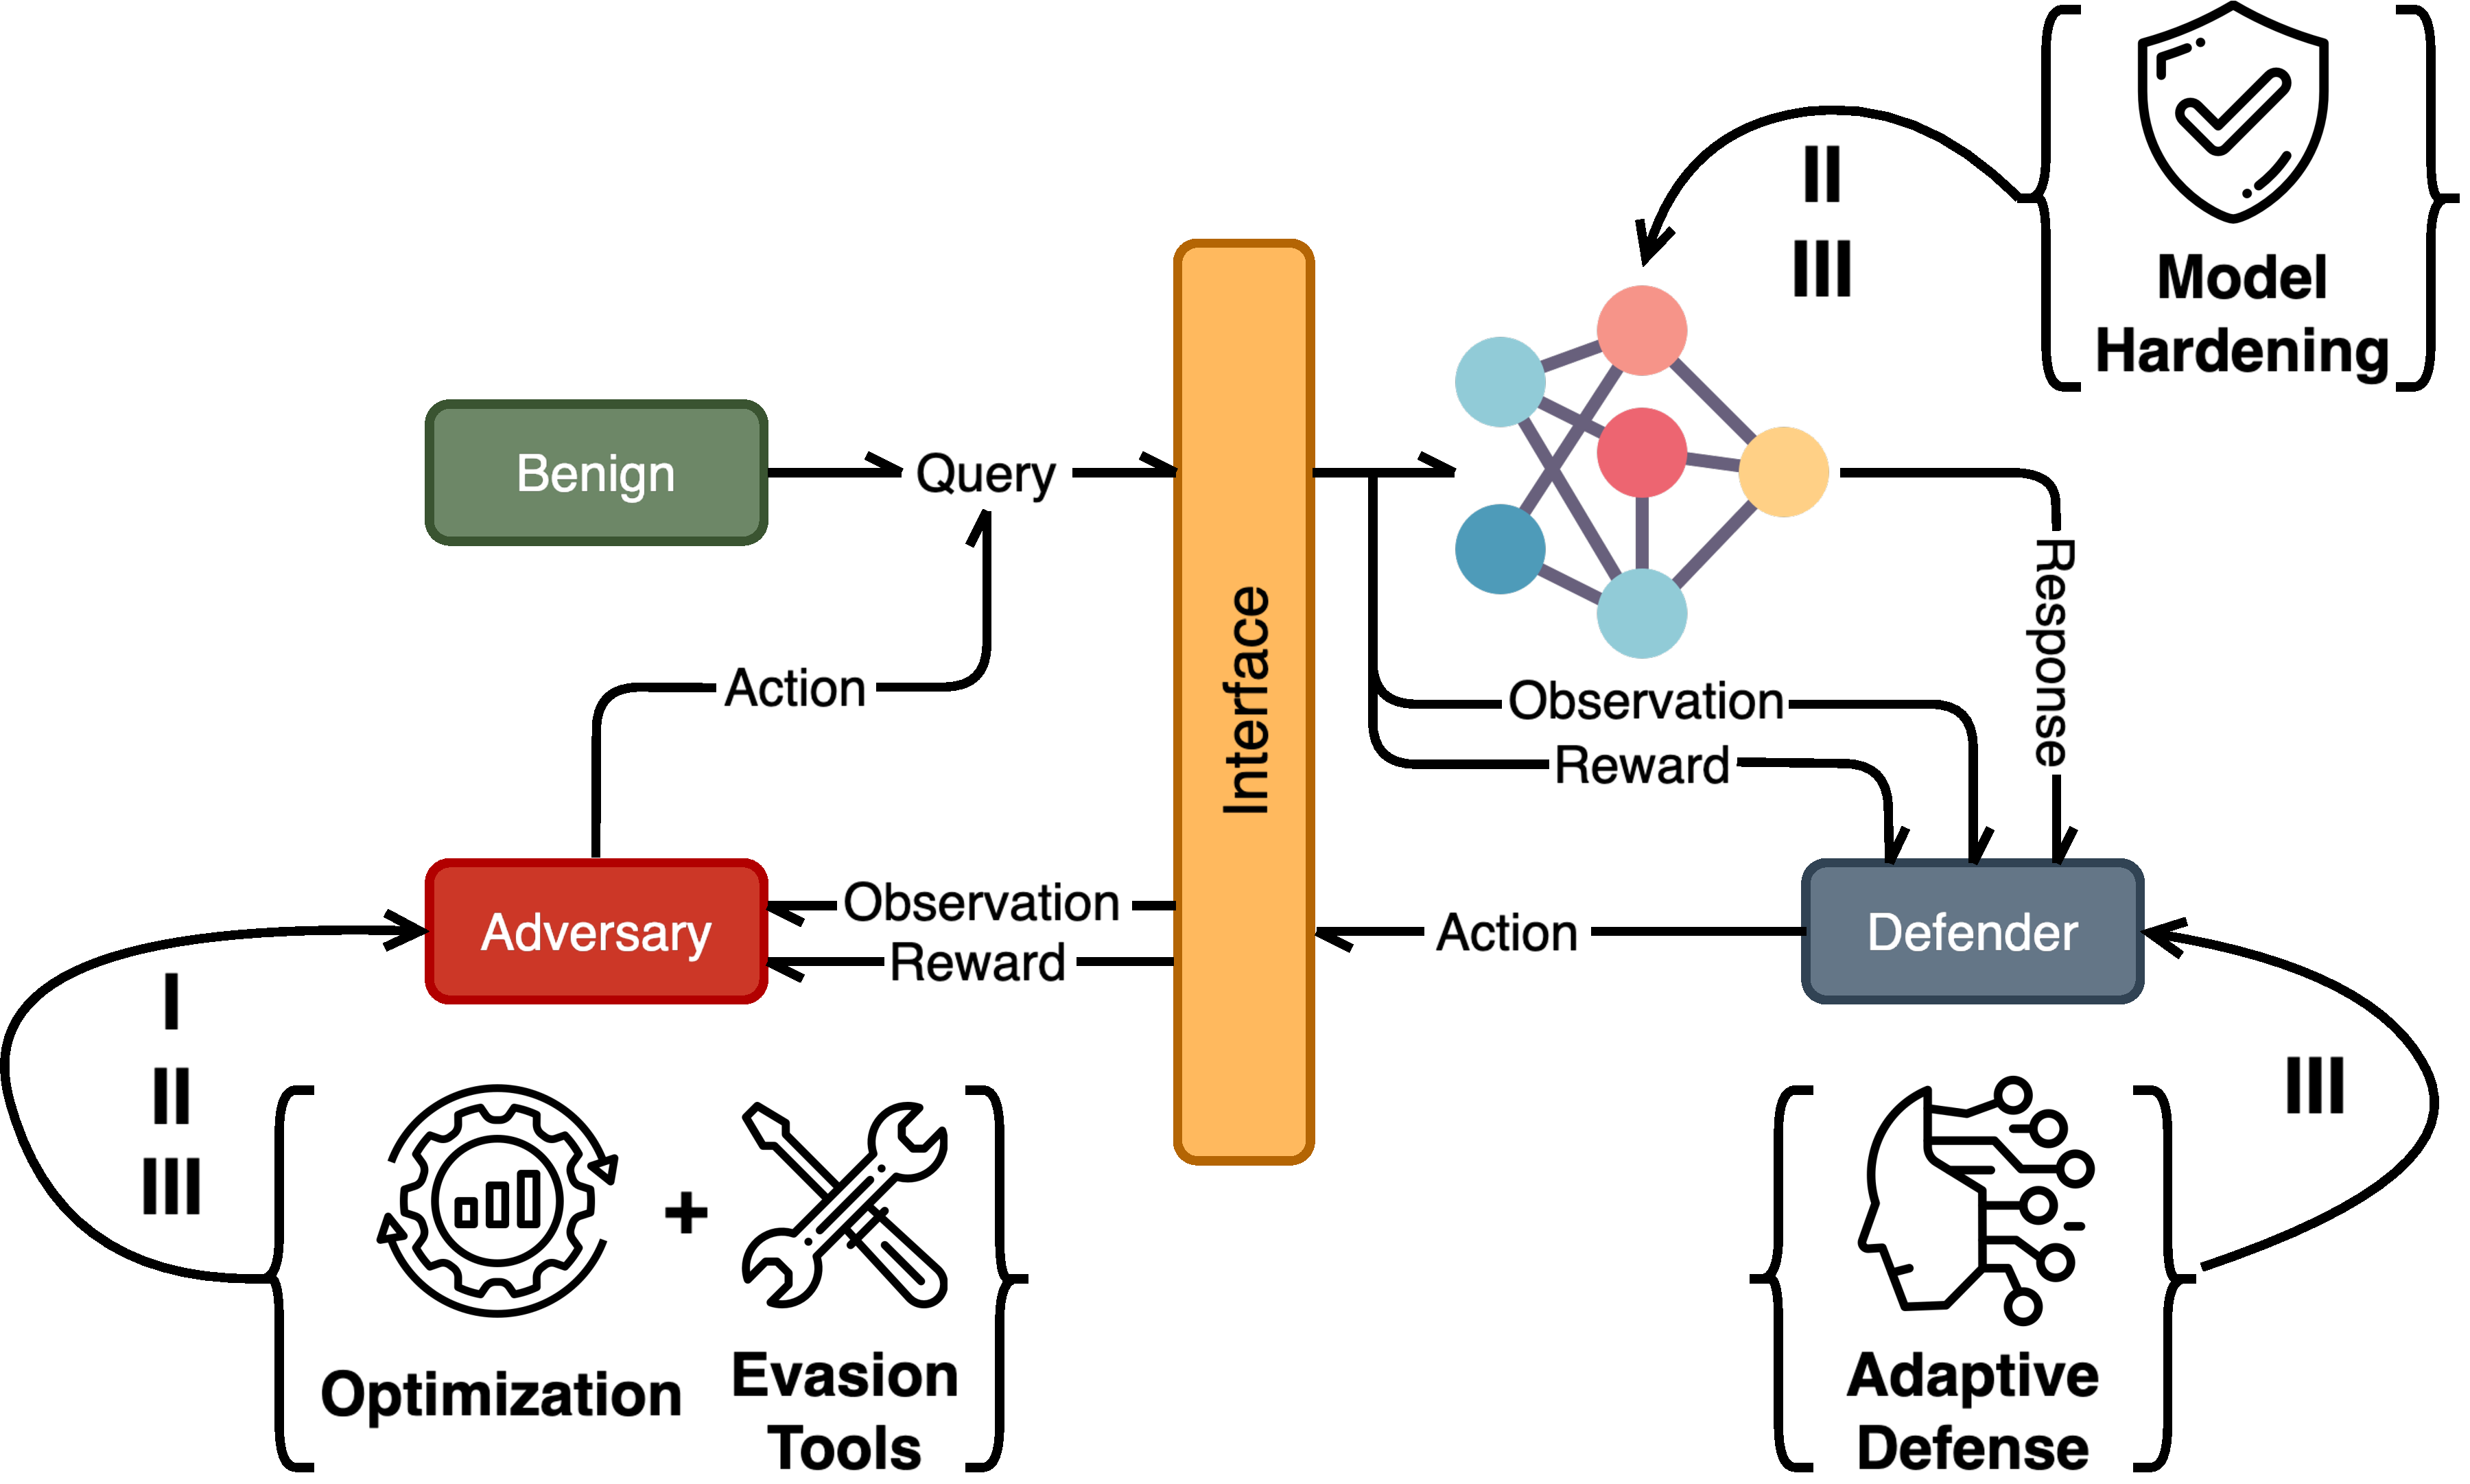
\includegraphics[width=0.99\textwidth]{pillars.pdf}
    \caption{Schematic depiction of an environment that encompasses attacks and defenses on a black-box AI model, and all the agents involved. We indicate where our three works (I, II, III) are situated with respect to each component or agent.}
    \label{fig:pillars}
\end{figure}

As previously presented in this introduction, the core of this dissertation is comprised of three major works on the security and robustness of AI-based systems against adversarial attacks.
These three works have several common underpinnings and build naturally upon each other.
To situate them in the broader \gls{AML} landscape, \autoref{fig:pillars} depicts an overview of a typical environment for black-box attack and defenses, as well as what is the focus in each of our works.
Our attack against Google reCAPTCHA v3, as an attack against a proprietary, real-world system, is in essene the optimization of an adversaril attack against the black-box system, through the information that this system divulges alone.
Our AutoRobust paper takes this a step further.
As the owners now of the detection model, we employ the process of optimizing attacks through the problem space to adversarially train the model.
Finally, our third work integrates all the above.
It optimizes attacks and their evasion tools, it hardens models againt evasion, and adds furthermore another defensive layer, namely active and adaptive defenses.

Besides these three major works, during my PhD trajectory I have pursued a wide range of research questions, in collaboration with other colleagues from KU Leuven and abroad.
I had the privilege to do a research visit in King's College London and University College London, a period and opportunity fundamental to my growth as a researcher and a person.
During this time I have also participated in several research projects and co-authored a book chapter, all falling under the cybersecurity and \gls{AML} umbrellas.
Below, I summarize my activities relevant to this dissertation that have also resulted in publications:

\textbf{AutoAttacker: A Reinforcement Learning Approach for Black-box Adversarial Attacks.}
Our initial foray into generating adversarial examples with \gls{RL} was successful, and led to my first publication, a workshop paper accepted at Euro S\&P 2019.
In AutoAttacker, \gls{RL} agents learn how to operate around the black-box model by querying it, to effectively extract the underlying decision behaviour, and to undermine it successfully.
Notably, AutoAttacker was a first of its kind framework to employ \gls{RL} in generating adversarial examples, irrespective of the differentiability of the underlying model, making the approach robust towards common defenses like gradient obfuscation or masking.

\begin{myleftbar}
\fullcite{tsingenopoulos2019autoattacker}
\end{myleftbar}

\textbf{Adaptive Malware Control: Decision-Based Attacks in the Problem Space of Dynamic Analysis}

In this work, we redefine adversarial attacks on malware behavior so that they can be performed directly by the original binary and thus obviate the need to compute gradients through feature representations.
We theoretically prove that this can occur even in the fully black-box case where only the final, hard-label decision is disclosed.
Furthermore, we empirically evaluate our approach by training state-of-the-art sequence models for detecting malware behavior, constructing several malware manipulation environments, and training a host of \gls{RL} agents on them that learn evasive policies through interaction.
Finally, we utilize the adversarial behavior learned by the RL agents to adversarially train the original detection models and we show that while an indispensable approach, the degree of robustness it imparts can be deceptive; especially when we consider adversaries with broader action sets.
This work was accepted for publication in the 1st Workshop on Robust Malware Analysis (WoRMA 2022) co-located with AsiaCCS 2022.

\begin{myleftbar}
\fullcite{tsingenopoulos2022adaptive}
\end{myleftbar}

\textbf{Position Paper: On Advancing Adversarial Malware Generation Using Dynamic Features}
In the same workshop, we also published a position paper on adversarial malware.
We conduct a critical review of existing adversarial attacks against malware detection, and conclude that current research focuses mainly on evasion techniques against static analysis; generating adversarial Windows samples to evade dynamic analysis remains largely unexplored.
In the context of black-box attack scenarios, we investigate an adversary's potential to carry out practical transformations in order to influence behavioral features observed by ML systems and security products. Moreover, we investigate the range of dynamic behavior transformations and identify critical properties and associated challenges that relate to feasibility, automation, technical costs and detection risks.
Through this discussion, we propose solutions to important challenges and present promising paths for future research on evasive malware under dynamic analysis.

\begin{myleftbar}
\fullcite{shafiei2022position}
\end{myleftbar}

\textbf{Adversarial Machine Learning}
Furthermore, with several colleagues we co-authored a book chapter on \gls{AML}.
While other chapters chapters in the book study the application of ML solutions to cybersecurity, in this chapter we study \gls{AML} as a field of study concerned with the security of ML algorithms when faced with attackers.
Likewise, \gls{AML} enjoys remarkable interest from the community, with a large body of works that either propose attacks against machine learning algorithms, or defenses against adversarial attacks.
In particular, adversarial attacks have been mounted in almost all applications of machine learning.
Here, we aim to systematize \gls{AML}, with a pragmatic focus on common computer security applications. Without assuming a strong background in machine learning, we also introduce the basic building blocks and fundamental properties of \gls{AML}.
This study is therefore accessible both to a security audience without in-depth knowledge of ML and to a ML audience.

\begin{myleftbar}
\fullcite{hernandez2022adversarial}
\end{myleftbar}

% \textbf{Chained Anomaly Detection Models for Federated Learning: An Intrusion Detection Case Study}
% The major challenge that we address in this work is that in a federated learning setup, an adversary has many more opportunities to poison one of the local machine learning models with malicious training samples, thereby influencing the outcome of the federated learning and evading detection.
% We present a solution where contributing parties in federated learning can be held accountable and have their model updates audited.
% We describe a permissioned blockchain-based federated learning method where incremental updates to an anomaly detection machine learning model are chained together on the distributed ledger.
% By integrating federated learning with blockchain technology, our solution supports the auditing of machine learning models without the necessity to centralize the training data.
% Experiments with a realistic intrusion detection use case and an autoencoder for anomaly detection illustrate that the increased complexity caused by blockchain technology has a limited performance impact on the federated learning, varying between 5 and 15\%, while providing full transparency over the distributed training process of the neural network.
% Furthermore, our federated learning solution can be generalized and applied to more sophisticated neural network architectures and other use cases.

% \begin{myleftbar}
% \fullcite{preuveneers2018chained}
% \end{myleftbar}

% \textbf{Resource Usage and Performance Trade-offs for Machine Learning Models in Smart Environments}
% Finally, we perform a study on multi-objective optimization for ML models, where the best performing model, its architecture and parameters for a given task are ideally automatically determined through a hyperparameter tuning process.
% At the same time, edge computing is an emerging distributed computing paradigm that aims to bring computation and data storage closer to the location where they are needed to save network bandwidth or reduce the latency of requests.
% The challenge we address in this work is that hyperparameter tuning does not take into consideration resource trade-offs when selecting the best model for deployment in smart environments.
% The most accurate model might be prohibitively expensive to computationally evaluate on a resource constrained node at the edge of the network.
% We propose a multi-objective optimization solution to find acceptable trade-offs between model accuracy and resource consumption to enable the deployment of ML models in resource constrained smart environments.
% We demonstrate the feasibility of our approach by means of an anomaly detection use case.
% Additionally, we evaluate the extent that transfer learning techniques can be applied to reduce the amount of training required by reusing previous models, parameters and trade-off points from similar settings.

% \begin{myleftbar}
% \fullcite{preuveneers2020resource}
% \end{myleftbar}

\section{Dissertation Outline}

The remainder of this dissertation is structured as follows:
We begin by introducing the necessary background knowledge on \gls{AML} and \gls{RL}, where for \gls{RL} we further introduce common algorithms, multi-agent environments, and its relevance for cybersecurity use-cases in Chapter \ref{ch:background}.
In Chapter \ref{ch:recaptcha} we present our first work, the RL-based attack that manages to succdessfuly bypass detection by Google reCAPTCHA v3.
In Chapter \ref{ch:autorobust} we introduce AutoRobust, our methodology of hardening malware detection models against evasion through the problem space.
In Chapter \ref{ch:markovgames} we investigate the confluence of adaptive attacks and defenses, and as their composition, we introduce our Adversarial Markov Games (AMG) framework.
Finally, in Chapter \ref{ch:conclusion} we conclude the dissertation by summarizing our key contributions and insights on the domain, and discuss possible and unexplored paths for future research.
% Some dummy code to get at least 1 entry in the nomenclature.
% \nomenclature{$\Theta$}{A nice symbol}
% Introducing some symbol: $\Theta$.

%%%%%%%%%%%%%%%%%%%%%%%%%%%%%%%%%%%%%%%%%%%%%%%%%%
% Keep the following \cleardoublepage at the end of this file, 
% otherwise \includeonly includes empty pages.
\cleardoublepage

% vim: tw=70 nocindent expandtab foldmethod=marker foldmarker={{{}{,}{}}}
